	\begin{figure}[H]
			\begin{minipage}[b]{0.49\textwidth}
				(a)
				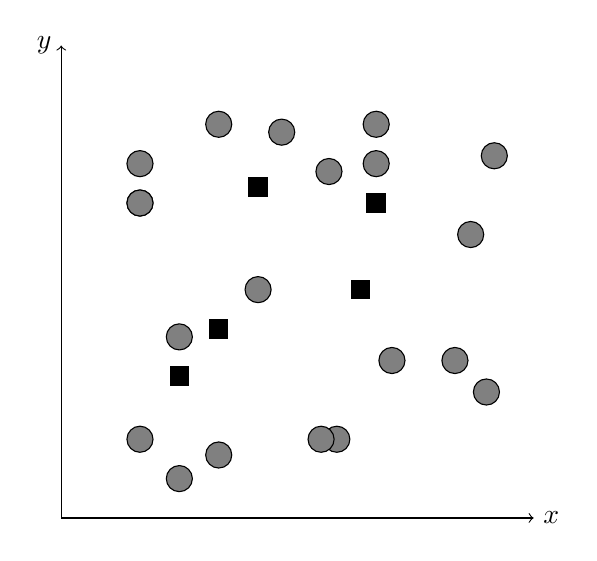
\begin{tikzpicture}
					\draw [->] (0,0,0) -- (6,0,0) node [at end, right] {$x$};
					\draw [->] (0,0,0) -- (0,6,0) node [at end, left] {$y$};
					\node [black,circle,draw,fill=gray](s) at (1,1,0){};
					\node [black,circle,draw,fill=gray](s) at (2,0.8,0){};
					\node [black,circle,draw,fill=gray](s) at (1.5,0.5,0){};
					\node [black,circle,draw,fill=gray](s) at (4,5,0){};
					\node [black,circle,draw,fill=gray](s) at (2,5,0){};
					\node [black,circle,draw,fill=gray](s) at (1,4.5,0){};
					\node [black,circle,draw,fill=gray](s) at (3.5,1,0){};
					\node [black,circle,draw,fill=gray](s) at (1,4,0){};
					\node [black,circle,draw,fill=gray](s) at (5.4,1.6,0){};
					\node [black,circle,draw,fill=gray](s) at (2.5,2.9,0){};
					\node [black,circle,draw,fill=gray](s) at (1.5,2.3,0){};
					\node [black,circle,draw,fill=gray](s) at (4.2,2,0){};
					\node [black,circle,draw,fill=gray](s) at (5,2,0){};
					\node [black,circle,draw,fill=gray](s) at (4,4.5,0){};
					\node [black,circle,draw,fill=gray](s) at (3.3,1,0){};
					\node [black,circle,draw,fill=gray](s) at (1,4,0){};
					\node [black,circle,draw,fill=gray](s) at (3.4,4.4,0){};
					\node [black,circle,draw,fill=gray](s) at (2.8,4.9,0){};
					\node [black,circle,draw,fill=gray](s) at (5.5,4.6,0){};
					\node [black,circle,draw,fill=gray](s) at (5.2,3.6,0){};
					
					\node [draw,fill=black](s) at (2,2.4,0){};
					\node [draw,fill=black](s) at (2.5,4.2,0){};
					\node [draw,fill=black](s) at (3.8,2.9,0){};
					\node [draw,fill=black](s) at (1.5,1.8,0){};
					\node [draw,fill=black](s) at (4,4,0){};
					
				\end{tikzpicture}
			\end{minipage}
			\begin{minipage}[b]{0.49\textwidth}
				(b)
				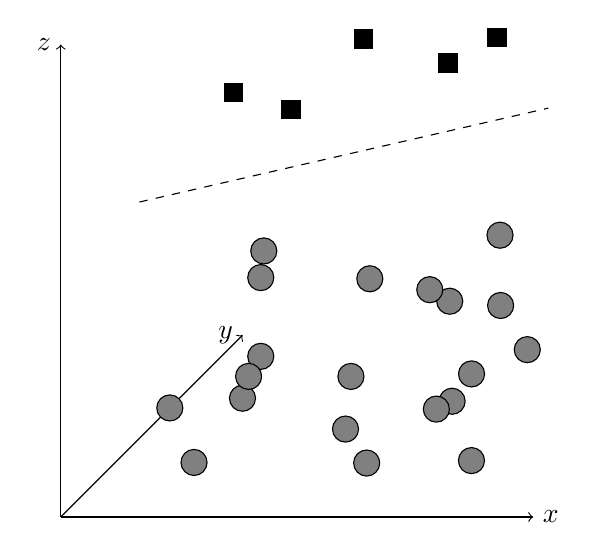
\begin{tikzpicture}
					\draw [->] (0,0,0) -- (6,0,0) node [at end, right] {$x$};
					\draw [->] (0,0,0) -- (0,6,0) node [at end, left] {$z$};
					\draw [->] (0,0,0) -- (0,0,-6) node [at end, left] {$y$};
					
					\node [black,circle,draw,fill=gray](s) at (1,1,-1){};
					\node [black,circle,draw,fill=gray](s) at (2,1.2,-0.8){};
					\node [black,circle,draw,fill=gray](s) at (1.5,0.5,-0.5){};
					\node [black,circle,draw,fill=gray](s) at (4,0.2,-5){};
					\node [black,circle,draw,fill=gray](s) at (2,1.1,-5){};
					\node [black,circle,draw,fill=gray](s) at (1,1.8,-4.1){};
					\node [black,circle,draw,fill=gray](s) at (3.5,0.3,-1){};
					\node [black,circle,draw,fill=gray](s) at (1,0.5,-4){};
					\node [black,circle,draw,fill=gray](s) at (4.6,0.1,-1.6){};
					\node [black,circle,draw,fill=gray](s) at (2.5,0,-2.9){};
					\node [black,circle,draw,fill=gray](s) at (1.5,0.9,-2.3){};
					\node [black,circle,draw,fill=gray](s) at (4.2,0.7,-2){};
					\node [black,circle,draw,fill=gray](s) at (4,0.6,-2){};
					\node [black,circle,draw,fill=gray](s) at (4,2,-4.1){};
					\node [black,circle,draw,fill=gray](s) at (3.3,1.4,-1){};
					\node [black,circle,draw,fill=gray](s) at (1,1.5,-4){};
					\node [black,circle,draw,fill=gray](s) at (3.4,1.2,-4){};
					\node [black,circle,draw,fill=gray](s) at (2.8,1,-4.9){};
					\node [black,circle,draw,fill=gray](s) at (3.6,0.2,-4.2){};
					\node [black,circle,draw,fill=gray](s) at (4.2,1.3,-3.6){};
					
					\node [draw,fill=black](s) at (2,4.25,-2.4){};
					\node [draw,fill=black](s) at (2.5,4.72,-3.5){};
					\node [draw,fill=black](s) at (3.8,4.65,-2.9){};
					\node [draw,fill=black](s) at (1.5,4.7,-1.8){};
					\node [draw,fill=black](s) at (4,4.55,-4){};
					
					\draw[dashed] (1,4,0) -- (6,5,-0.5);
				\end{tikzpicture}
			\end{minipage}
			\centering
			\caption{(a) Abbildung von möglichen, Objektklassen im zweidimensionalen Raum. Die Formen stellen jeweils Klassen dar, wie zum Beispiel die Klassen Hund und Person. (b) Darstellung der in a gezeigten Objektklassen im dreidimensionalen Raum. Die gestrichelte Linie deutet eine lineare Trennung an.}
			\label{fig: kerneltrick}
	\end{figure}